\documentclass[]{llncs} % "you can ignore this hint if your document works"
\usepackage{makeidx}
\usepackage{graphicx}
\usepackage{makecell}
\usepackage{float}
\begin{document}
\addtocmark{Southern Methodist University}

\title{Machine Learning Predicts Aperiodic Laboratory Earthquakes}
\author{Olha Tanyuk, Daniel Davieau, Charles South \and Daniel W. Engels}
\institute{Southern Methodist University, Dallas TX 75205, USA \newline otanyuk@mail.smu.edu, danieldavieau@mail.smu.edu, csouth@mail.smu.edu, dwe@lyle.smu.edu }


\maketitle
\begin{abstract}
%In this paper we find a pattern of aperiodic seismic signals that precede earthquakes at any time in a laboratory earthquake’s cycle using a small window of time.  We use data collected from an experiment which exhibits similar behavior to natural earthquakes, so the same approach may work in predicting the timing of natural earthquakes. We apply machine learning to a data set that comes from a classic laboratory experiment having several stick-slip displacements (earthquakes), a type of experiment which has been studied in depth as a simulation of seismologic faults for decades. We show that by listening to the acoustic signal emitted by the laboratory experiment a machine learning algorithm can predict the time remaining before it fails. These predictions are based only on the the acoustic signal and not its history. \par
In this paper we find a pattern of aperiodic seismic signals that precede earthquakes at any time in a laboratory earthquake’s cycle using a small window of time.  We use a data set that comes from a classic laboratory experiment having several stick-slip displacements (earthquakes), a type of experiment which has been studied as a simulation of seismologic faults for decades. This data exhibits similar behavior to natural earthquakes, so the same approach may work in predicting the timing of them. Here we show that by applying random forest regression to the acoustic signal emitted by a laboratory fault, we can predict the time remaining before failure with 1.61 seconds mean absolute error at any moment of earthquake’s cycle. These predictions are based solely on the acoustical signal's statistical features derived from the local, moving 0.3 second time windows and do not make use of its history. Essential improvements in providing new understanding of fault physics may be brought by applying this technique to acoustic seismic data.\par

%In this paper we present a method for predicting the timing of laboratory earthquakes using machine learning. If a similar approach can be applied to improve natural earthquake prediction it will save lives. We use data collected from a laboratory experiment which exhibits similar behavior to natural earthquakes. We train a machine learning algorithm using half of the data, then predict using the other half. We compare predicted versus actual timings to measure the algorithm's accuracy. The result shows that the timing of laboratory earthquakes can be predicted up to 16 seconds in advance with 71\% accuracy. The method and result demonstrates that machine learning can help if it can be scaled from the laboratory experiment to natural earthquakes. \par
\end{abstract}

\section{Introduction}
Earthquakes cause mass destruction and loss of life. A traditional method to predict earthquakes is to look to past recurrence intervals. Because the recurrences are not constant, predictions can only be made within broad time windows. One such model predicted that a strong earthquake would occur between 1985 and 1993 in the Parkfield California area but no significant event actually occurred until 2004 \cite{Jackson}. \par
Another way to predict earthquakes are based on changes in land elevation, ground water levels, animal behavior or foreshocks \cite{PNSN}. There are couple examples when this method of prediction worked. The segment of the San Andreas Fault that broke in the 1989 magnitude 7.1  (see section 2 Earthquakes for more details about magnitude) Loma Prieta or "World Series" earthquake had been identified by the USGS (U.S. Geological Survey) as one of the more likely segments of the San Andreas to rupture. Magnitude 5+ earthquakes 2 and 15 months before the damaging earthquake were treated as possible foreshocks, and the USGS issued 5-day Public Advisories through the California Office of Emergency Services \cite{PNSN}. Even in areas where foreshocks are fairly common, there is no way of distinguishing a foreshock from an independent earthquake \cite{PNSN}. In the Pacific Northwest, there is no evidence of foreshock activity for most historic earthquakes \cite{PNSN}.\par
One well-known successful earthquake prediction was for the Haicheng, China earthquake of 1975, when an evacuation warning was issued the day before a magnitude 7.3 earthquake \cite{PNSN}. In the preceding months changes in land elevation and in ground water levels, widespread reports of peculiar animal behavior, and many foreshocks had led to a lower-level warning \cite{PNSN}. An increase in foreshock activity triggered the evacuation warning \cite{PNSN}. Unfortunately, most earthquakes do not have such obvious precursors \cite{PNSN}. In spite of their success in 1975, there was no warning of the 1976 Tangshan earthquake, magnitude 7.6, which caused an estimated 250,000 fatalities \cite{PNSN}.\par
Advances in instrumentation quality and density have fostered hope that progress can be made in forecasting. These advances have led to discoveries of previously unidentified slip processes such as slow slips. Slow Slip Earthquakes (SSE) are fault behaviors that occur slowly enough to make them undetectable without instrumentation. They do not cause immediate widespread destruction like regular earthquakes do. They occur near the boundaries of large earthquake rupture zones \cite{Slip}. There is evidence to suggest that there is a relationship between slow slip earthquakes and more noticeable regular earthquakes \cite{SlowSlip}. \par
Researchers imitate natural slow slip earthquakes in the laboratory by placing rocky material between steel blocks and applying shear stress to induce slipping. Recent improvements in the instruments \cite{kaggle} used to measure signals have enabled the collection of larger volume and more akin to natural earthquake data. However, processing the data and detecting patterns in it has become more difficult. Methods to detect patterns of aperiodic seismic signals that precede earthquakes are presented in this paper. We use acoustic data provided by the Los Alamos National Laboratory (LANL) as part of a 2019 Kaggle competition \cite{kaggle} which represents laboratory slow-slip earthquakes. The data is very aperiodic and more akin to natural earthquakes than the data LANL studied earlier in 2017 \cite{kaggle}. We demonstrate that random forest regression can be used to detect patterns in the data that and predict laboratory earthquakes with mean absolute error of 1.61 seconds. Given seismic signal data with considerably more aperiodic slow-slip laboratory earthquake failures, we predict time remaining before failure at any time in the slip cycle based solely on acoustical signal's statistical features derived from the small, local, moving time windows and do not make use of its history.\par
The results of this experiment are potentially applicable to the field of real world earthquakes \cite{Bertrand}. Essential improvements in providing new understanding of fault physics may be brought by applying this technique to acoustic seismic data. Other potential applications include avalanche prediction, landslides and failure of machine parts \cite{Bertrand}. \par


%Earthquakes cause mass destruction and loss of life. Traditional earthquake prediction methods have relied on recurrence interval based models. Because the recurrences are not constant predictions can only be made within decade spanning time windows. One such model predicted that a magnitude 6 earthquake would occur between 1985 and 1993 in the Parkfield California area but no significant event occurred until 2004 \cite{Jackson}. \par
%
%Researchers imitate natural earthquakes in the laboratory by placing rocky material between steel blocks and applying shear stress to induce slipping. Recent improvements in the instruments \cite{Bertrand} used to measure signals have enabled the collection of larger volume data from more realistic and unpredictable laboratory earthquakes. However processing the data and detecting patterns in it has become more difficult to work with. In this paper we demonstrate that machine learning can be used to detect patterns and make predictions from realistic, unpredictable laboratory earthquake data \cite{kaggle}.\par
%
%We use data which was collected by the Los Alamos National Laboratory and provided to the public via a Kaggle competition \cite{kaggle}. It consists of 629 million acoustic signal observations and an accompanying record of the time remaining until a laboratory earthquake (failure) occurred \cite{Bertrand}. We calculate additional statistical measures such as variance, kurtosis and skew for each observation. We use half of the data to train a machine learning algorithm. With the remaining half of the data, using only the acoustic signal as input we calculate a prediction of the time remaining until failure. We measure  accuracy by comparing the predicted to actual remaining time to failure from the original data. \par
%
%The result shows that the timing of laboratory earthquakes can be predicted up to 16 seconds in advance with 71 percent accuracy.\par
%
%%Conclusion
%The data, hardware and software allows us to predict impending laboratory earthquakes. However we only know 8-16 seconds before failure. Therefore practical applications may be limited. This may prove useful but only applies to laboratory experiments. This could be used in industry perhaps in researching materials for wallboard, machine parts and others.\par

\section{Earthquakes}
An earthquake is the shaking of the Earth's surface caused by sudden releases of energy in the lithosphere that creates seismic waves. It happens when two blocks of the earth suddenly slip past one another. The surface where they slip is called the fault or fault plane \cite{Wald}. The location below the earth’s surface where the earthquake starts is called the hypocenter, and the location directly above it on the surface of the earth is called the epicenter \cite{Wald}. \par
Smaller earthquakes that happen in the same location as a larger earthquake that follows are called fore shocks. Scientists can’t determine whether an earthquake is a foreshock until the larger earthquake happens \cite{Wald}. The largest, main earthquake is called the mainshock \cite{Wald}. Mainshocks always have aftershocks that follow, smaller earthquakes that occur afterwards in the same place as the mainshock \cite{Wald}. Depending on the size of the mainshock, aftershocks can continue for weeks, months, and even years after the mainshock \cite{Wald}.\par
The earth has four major layers: the inner core, outer core, mantle and crust \cite{Wald}. The crust and the top of the mantle make up a thin skin on the surface of our planet; this skin is not all in one piece; it is made up of many pieces like a puzzle covering the surface of the earth \cite{Wald}. These puzzle pieces are called tectonic plates, and the edges of the plates are called the plate boundaries. Tectonic plates move slowly and continuously; sliding past and bumping into each other. The plate boundaries are made up of many faults, and most of the earthquakes around the world occur on these faults \cite{Wald}. Because the edges of the plates are not smooth they can get stuck while the rest of the plate keeps moving \cite{Wald}. Finally, when the plate has moved far enough, the edges unstick on one of the faults and there is an earthquake \cite{Wald}. \par
While the edges of faults are stuck together, and the rest of the block is moving, the energy that would normally cause the blocks to slide past one another is being stored up \cite{Wald}. When the force of the moving blocks finally overcomes the friction of the jagged edges of the fault and it unsticks and all of the stored energy is released \cite{Wald}. The energy radiates outward from the fault in all directions in the form of seismic waves, those waves shake the earth as they move through it, and when the waves reach the earth’s surface, they shake the ground and anything on it \cite{Wald}. \par
The size of an earthquake depends on the size of the fault and the amount of slip on the fault, but that’s not something scientists can simply measure with a measuring tape since faults are many kilometers deep beneath the earth’s surface \cite{Wald}. The strength of the shaking from an earthquake diminishes with increasing distance from the earthquake's source, so the strength of the shaking at the surface from an earthquake that occurs 500km below the surface can considerably less than if the same earthquake had occurred 20 km below the surface \cite{Wald}. The size of the earthquake is called its magnitude. The Richter Scale (ML) is what most people have heard about(scale range from 0 to 9), but in practice it is not commonly used anymore, except for small earthquakes recorded locally, for which ML and short-period surface wave magnitude (Mblg) are the only magnitudes that can be measured \cite{Hayes}. For all other earthquakes, the moment magnitude (Mw) scale is a more accurate measure of the earthquake size \cite{Hayes}. Moment Magnitude (MW) is based on physical properties of the earthquake derived from an analysis of all the wave forms recorded from the shaking \cite{Hayes}. First the seismic moment is computed, and then it is converted to a magnitude designed to be roughly equal to the Richter Scale in the magnitude range where they overlap \cite{Hayes}. Another way to measure the size of an earthquake is to compute how much energy it released \cite{Hayes}. The amount of energy radiated by an earthquake is a measure of the potential for damage to man-made structures \cite{Hayes}. The energy can be converted into yet another magnitude type called the Energy Magnitude (Me) \cite{Hayes}. \par
Slow Slip Earthquakes (SSE) are fault behaviors that occur slowly enough to make them undetectable without instrumentation. They do not cause immediate widespread destruction like regular earthquakes do. They occur near the boundaries of large earthquake rupture zones \cite{Slip}. Most SSE's have been observed near the downdip limit of the seismogenic zone at depths of 25–45 km, but in well-instrumented areas they have also been detected at shallow depths (less than 10 km), updip of large earthquake ruptures \cite{Slip}. SSE's at tectonic boundaries probably occur at the plate interface, and therefore should be controlled by the frictional properties and conditions that characterize fault zones \cite{Slip}. For deep slow slip events, laboratory testing of natural material under in situ conditions is not feasible at present \cite{Slip}.  


\section{Los Alamos National Laboratory's Findings}
In 2017 Los Alamos National Laboratory (LANL) researchers discovered a way to successfully predict Slow Slip Earthquakes (SSE) in a laboratory experiment that simulates natural conditions. The team trained a computer to pinpoint and analyze quasi‐periodic seismic and acoustic signals emitted during the movements along the fault. They processed massive amounts of data and identified a particular sound pattern previously thought to be noise that precedes an earthquake. The team was able to characterize the time remaining before a laboratory earthquake at all times using a time window of 1.8 sec of the data to make each prediction with 89\% coefficient of determination \cite{LANLNews}. This result was achieved using a Random Forest Regression machine learning technique and quasi‐periodic data. \par
In the lab, the team imitated a real earthquake using steel blocks interacting with rocky material to cause slipping that emitted seismic sounds. An accelerometer recorded the acoustic emission emanating from the sheared layers \cite{LANLNews}. For the first time, researchers discovered a pattern that accurately predicted when a laboratory earthquake would occur. The LANL team acknowledges that the characteristics of the lab experiment such as shear stress differ from natural earthquakes but the application of the analysis to the real world to validate their results is ongoing. This method can also be applied outside of seismology to support material failure research in other fields such as aerospace and energy \cite{LANLNews}. The lab results reveal that the fault does not fail randomly but in a predictable manner. The observations also demonstrate that the fault’s critical stress state which indicates when it might slip can be determined using exclusively an equation of state \cite{LANLNews}. So far seismologists and earth scientists have mostly relied on catalogs of historical data to try to characterize the state of faults. These catalogs contain a minute fraction of seismic data with portions discarded during analysis as useless noise. The authors discovered that hidden in the noise-like data are signals that inform them of the state of the fault much more precisely than catalogs \cite{LANLNews}. \par

\section{Random Forest Overview}
Random Forest (RF) is an ensemble machine learning technique capable of performing both regression and classification tasks using multiple decision trees and a statistical technique called bagging \cite{RandomForest}. Decision trees are predictive models that use a set of binary rules to calculate a target value \cite{RandomForest}. Each individual tree is a fairly simple model that has branches, nodes and leaves  \cite{RandomForest}. A sub section of the entire tree is called a branch or sub-tree. A Root Node represents the entire population or sample and this further gets divided into two or more homogeneous sets. Nodes that do not split are called Leaves. A decision tree is arriving at an estimate by asking a series of questions to the data, each question narrowing the possible values until the model gets confident enough to make a single prediction \cite{RandomForest}. The order of the questions (the questions asked are all in a True/False form) as well as their content are being determined by the model \cite{RandomForest}. Rather than just averaging the prediction of trees, a random forest uses two key concepts that give it the name random: \par
1. Random sampling of training observations when building trees.\par
2. Random subsets of features for splitting nodes.\par
In other words a random forest builds multiple decision trees and merges their predictions together to get a more accurate and stable prediction rather than relying on individual decision trees \cite{RandomForest}.\par
Each tree in a random forest learns from a random sample of the training observations \cite{RandomForest}. The samples are drawn with replacement (known as bootstrapping) which means that some samples will be used multiple times in a single tree \cite{RandomForest}. The idea is that by training each tree on different samples, although each tree might have high variance with respect to a particular set of the training data, overall, the entire forest will have lower variance but not at the cost of increasing the bias \cite{RandomForest}. \par
The fundamental idea behind a random forest is to combine the predictions made by many decision trees into a single model \cite{RandomForest}. Individually, predictions made by decision trees may not be accurate but combined together, the predictions will be closer to the true value on average \cite{RandomForest}.\par
Let's understand Random Forest step by step in below example:
Step 1: Samples are taken repeatedly from the training data so that each data point is having an equal probability of getting selected, and all the samples have the same size as the original training set \cite{RandomForest}.\par
Let's say we have the following data:\par
x= 0.1,0.5,0.4,0.8,0.6, y=0.1,0.2,0.15,0.11,0.13 where x is an independent variable with 5 data points and y is dependent variable \cite{RandomForest}.\par
Now bootstrap samples are taken with replacement from the above data set. n estimators is set to 3 (number of trees in random forest), then:\par
The first tree will have a bootstrap sample of size 5 (same as the original dataset), assuming it to be: \par
x1={0.5,0.1,0.1,0.6,0.6}\par
x2={0.4,0.8,0.6,0.8,0.1}\par
x3={0.1,0.5,0.4,0.8,0.8}\par
Step 2: A Random Forest Regressor model is trained at each bootstrap sample drawn in the above step, and a prediction is recorded for each sample \cite{RandomForest}.\par
Step 3: Now the ensemble prediction is calculated by averaging the predictions of the above trees producing the final prediction \cite{RandomForest}.\par

In our work training data is used to generate the RF model. The testing data is used to evaluate the performance of the RF model; this constitutes a fair measure of the RF performance because the testing data is independent from the training process (i.e. out of sample performance). It is very important to ensure that testing data does not leak into the training process \cite{Bertrand}. \par
The tree is given by a bootstrap re-sampling of the training data, which induces variation between the trees and mitigates the effect of outliers on the forest \cite{Bertrand}. To generate each node, we formulate a "yes"/"no" decision (corresponding to a split into left/right branches) operating on the data available at the current node. At each node, we select a random subset of the available features. From the selected features, we construct the decision that best predicts the time to failure \cite{Bertrand}. \par
The values used to evaluate predictions in our work are the coefficient of determination $r^2$ and mean absolute error ($MAE$) (Table 1). \par
\begin{table}
	\centering
	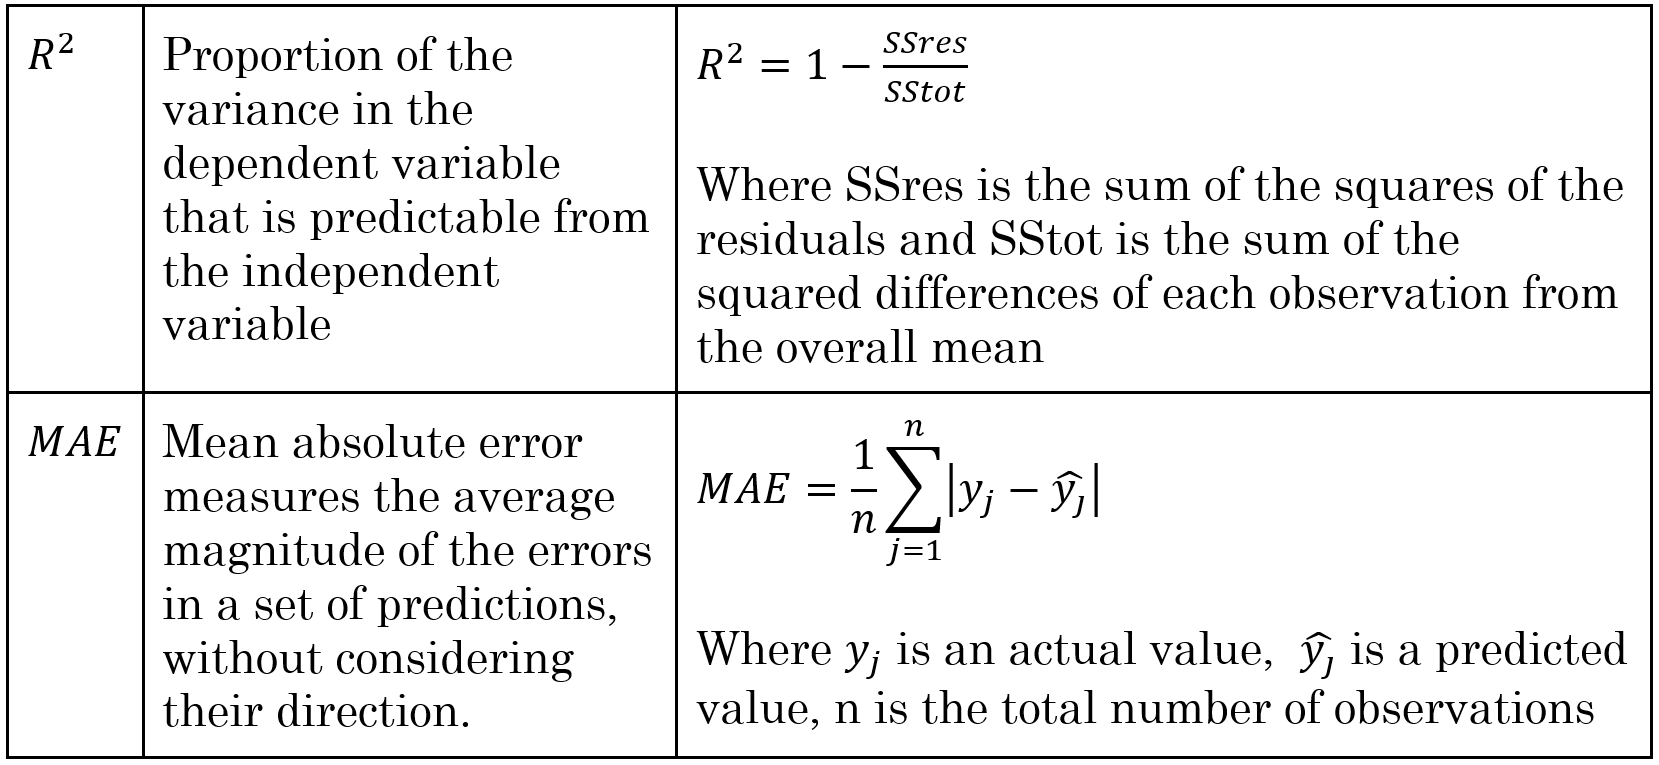
\includegraphics[width=.9\linewidth]{background}
	\caption{Statistical values used to evaluate predictions.}
	\label{fig:background}
\end{table}

\section{Data} 
\subsection{Data Generation Experimental Setup}
The laboratory system is a two‐fault configuration that contains fault gouge material submitted to double direct shear (Figure 1)\cite{kaggle}. \par
\begin{figure}[h]
	\centering
	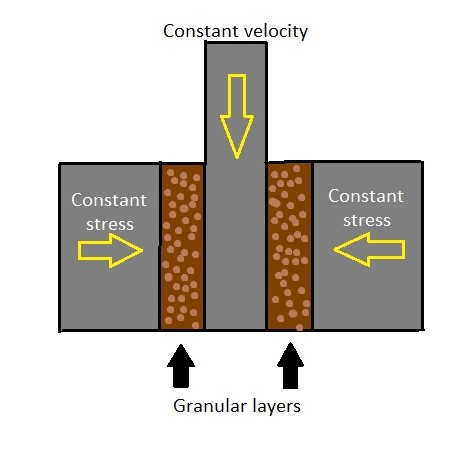
\includegraphics[width=.6\linewidth]{lab}
	\caption{Laboratory Earthquake Design}
	\label{fig:lab}
\end{figure}
Two fault gouge layers are sheared simultaneously while being subjected to a constant normal load and a prescribed shear velocity \cite{kaggle}. The laboratory faults fail in repetitive cycles of stick and slip that is meant to mimic the cycle of loading and failure on tectonic faults \cite{kaggle}. While the experiment is considerably simpler than a fault in the Earth it shares many physical characteristics \cite{kaggle}. \par

A driving piston displaces at a very constant velocity during the inter-event time and accelerates briefly when a slip occurs \cite{Bertrand}. An accelerometer records the acoustic emission emanating from the shearing layers \cite{Bertrand}. The steel blocks are extremely stiff therefore the deformation takes place largely in the gouge \cite{Bertrand}. Under a broad range of load and shear velocity conditions, the apparatus stick‐slips quasi‐periodically for hundreds of stress cycles during a single experiment and in general follows predictions from rate and state friction \cite{Bertrand}. The rate of impulsive precursors accelerates as failure approaches suggesting that upcoming laboratory earthquake timing could be predicted \cite{Bertrand}. \par

The experimental data has 16 earthquakes. The shortest time to failure is 1.5 seconds for the first earthquake, 7 seconds for the 7th and the longest is around 16 seconds. \par

\subsection{Data Exploration}
The data used in this work is a 157.275 second recording of seismic signals (ordered sequentially.) It was recorded at 4MHz hence 629,145,480 data points accompanied by the time remaining in seconds until the following lab earthquake. \par
The seismic signals are recorded using a piezoceramic sensor which outputs a voltage upon deformation by incoming seismic waves (henceforth we will use the term acoustic signal). The seismic data, which serves as the input to our analysis, is this recorded voltage, in integers. \par
% to prevent images from floating all over the place in the document: https://tex.stackexchange.com/questions/16207/image-from-includegraphics-showing-up-in-wrong-location
%\begin{table}
%	\begin{center}
%		\caption{Data Definitions}
%		\label{tab:DataDefinitions}
%		\begin{tabular}{ll}
%			\textbf{Acoustic Signal} & Voltage upon deformation by incoming seismic waves. \\
%			\textbf{Time To Failure} & The remaining time in seconds until an actual stick-slip failure occurred.  \\
%		\end{tabular}
%	\end{center}
%\end{table}
The \emph{Acoustic Signal} is the voltage upon deformation by incoming seismic waves. These signals are integers in the range [-5515 to 5444] with a mean of 4.52. The distribution of the acoustic signals has a very high peak and we see outliers in both directions (Figure 6). \par
The \emph{Time to Failure} is the remaining time in seconds until an actual stick-slip failure occurred. The minimum value is very close to zero (9.55039650e-05 seconds) and the maximum is 16 seconds. The distribution of the time to failure is right skewed (Figure 7). \par
The first five rows of the data are shown in Table 2. \par

\begin{table}
	\begin{center}
		\caption{The first five rows of the data}
		\label{tab:SampleData}
		\begin{tabular}{c|r} 
			\textbf{Acoustic Signal} & \textbf{Time to Failure}\\
			\hline
			12 & 1.469099998474121 \\ 
			6 & 1.469099998474121 \\ 
			8 & 1.469099998474121 \\ 
			5 & 1.469099998474121 \\ 
			8 & 1.469099998474121 \\ 
		\end{tabular}
	\end{center}
\end{table}

The acoustic signal shows huge fluctuations regularly just before each failure (Figure 2). It is also worth noting that failures can be predicted visually as cases when huge fluctuations in the signal are followed by smaller signals.\par
\begin{figure}
	\centering
	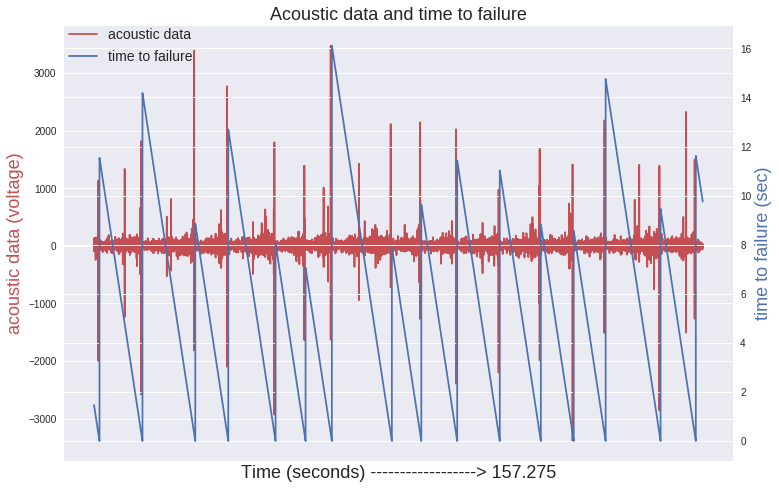
\includegraphics[width=.9\linewidth]{timeSeries}
	\caption{157.275 seconds of the data}
	\label{fig:timeseries}
\end{figure}

On a zoomed-in time plot (Figure 3) we see that the large acoustic signal oscillation at the 1.572 second mark is not at the exact time of the failure but just before it. There are trains of intense signal oscillations preceding the large one and some smaller ones after it.\par
\begin{figure}
	\centering
	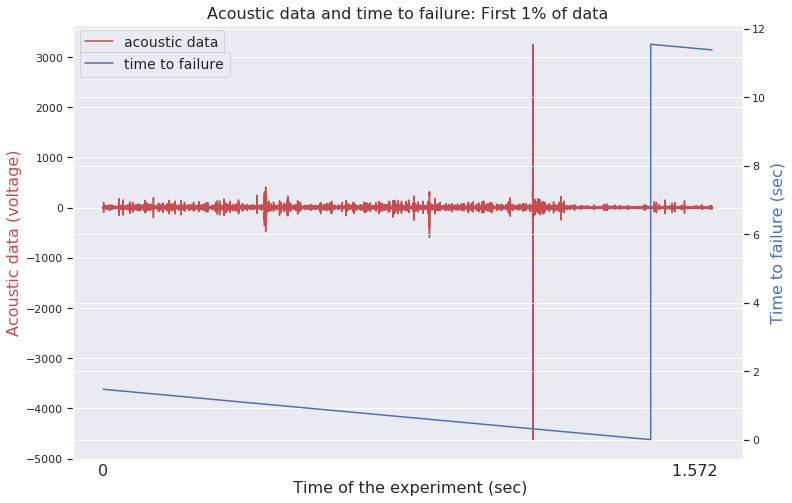
\includegraphics[width=.9\linewidth]{zoomedInTimePLot}
	\caption{1.572 seconds of data}
	\label{fig:zoomeInTimePlot}
\end{figure}

 A 1\% sample of the data (a histogram in Figure 4) shows that the voltage amplitude of acoustic precursors accelerates as failure approaches, suggesting that upcoming laboratory earthquake timing could be predicted. The red line indicates that a quake occurs when the time to failure approaches 0. \par
\begin{figure}
	\centering
	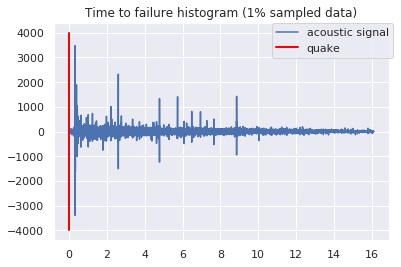
\includegraphics[width=.8\linewidth]{timeToFailureHistogram}
	\caption{1\% sample of the data histogram}
	\label{fig:timeToFailureHistogram}
\end{figure}

We found that more than 90\% of the high acoustic signal values (absolute value greater than 1000 voltages) are around 0.31 seconds before an earthquake (Figure 5). \par
\begin{figure}
	\centering
	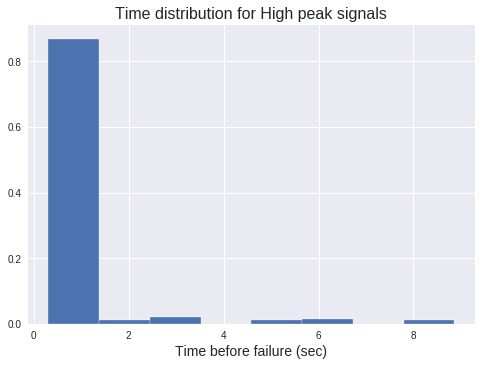
\includegraphics[width=.8\linewidth]{timeDistribution}
	\caption{The highest column represents 90\% of high acoustic signal values (absolute value greater than 1000 voltage).}
	\label{fig:timeDistribution}
\end{figure}

\begin{figure}
	\centering
	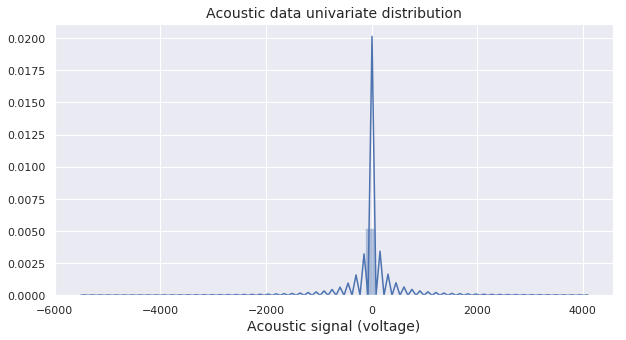
\includegraphics[width=.9\linewidth]{acousticDataDistribution}
	\caption{Univariate distribution of the acoustic signals}
	\label{fig:acousticDataDistribution}
\end{figure}

\begin{figure}
	\centering
	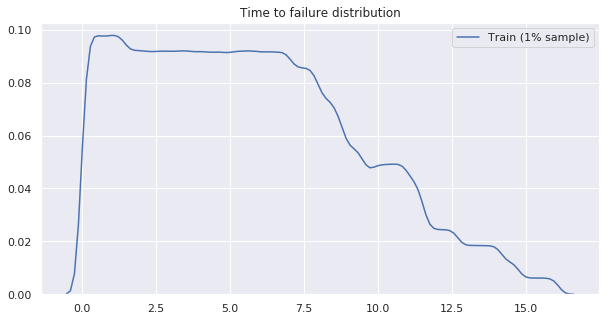
\includegraphics[width=.9\linewidth]{timeToFailureDistribution}
	\caption{Univariate distribution of the time to failure}
	\label{fig:timeToFailureDistribution}
\end{figure}
%\begin{figure}
%	\centering
%	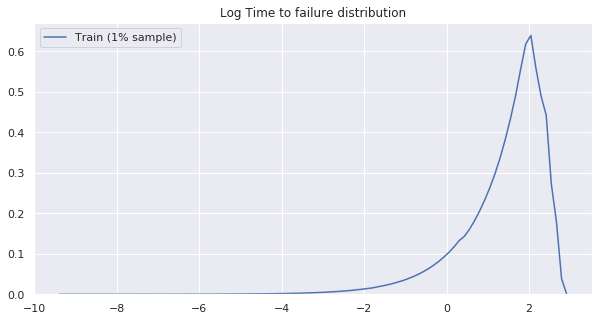
\includegraphics[width=.9\linewidth]{logTimeToFailureDistribution}
%	\caption{In this plot we can see that applying a logarithmic transform to the time to failure results in a left skewed distribution.}
%	\label{fig:logTimeToFailureDistribution}
%\end{figure}
%\begin{figure}
%	\centering
%	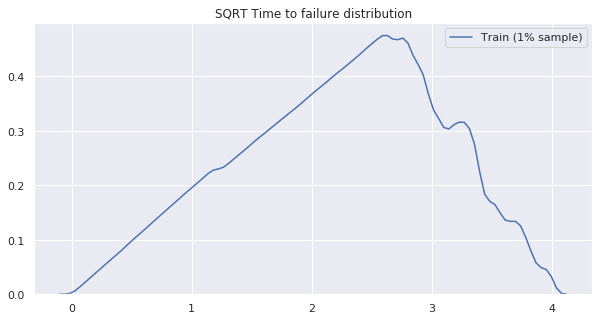
\includegraphics[width=.9\linewidth]{sqrtTimeToFailureDistribution}
%	\caption{ In this plot we can see that applying a square root transformation to the time to failure is still not normal but improved the distribution significantly. We used a square root transformation for normalization of the time to failure distribution.}
%	\label{fig:sqrtTimeToFailureDistribution}
%\end{figure}
\clearpage
\newpage
\section{Feature Engineering}
Working with quasi periodic seismic signals LANL achieved a 0.89 coefficient of determination. They divided the data into 1.8 second time windows and used a Random Forest technique. \cite{Bertrand}. The most important features in the LANL model were variance, kurtosis and threshold. \par
We used a similar approach in this study. Our goal is to predict the time remaining before the next failure using only moving time windows of the acoustic data. We divided the data into 0.3 second time windows (1,500,000 observations) which is small relative to the lab quake cycle which spans 8 to 16 seconds. As indicated in Figure 6; more than 90\% of high acoustic values (absolute value greater than 1000) are around 0.31 seconds before an earthquake therefore we divide our data by 0.3 second windows to reduce error at the end of the quake cycle. \par
Checking how sensitive our results are to the size of the time window (Figure 8) we find that the highest $r^2$ and smallest mean absolute error we were able to achieve is with 1.5M observations in each time window (0.3 seconds). \par
\begin{figure}
	\centering
	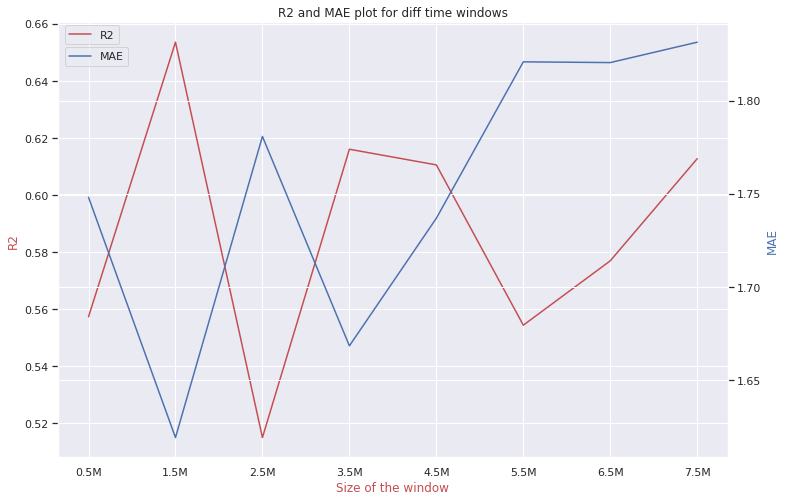
\includegraphics[width=.9\linewidth]{rSquaredandMAE}
	\caption{Model sensitivity to the size of the time window}
	\label{fig:rSquaredandMAE}
\end{figure}

Our resulting transformed data set consists of 419 time windows (0.3 seconds each).  From each time window we compute a set of 95 potentially relevant statistical features (e.g., mean, variance, kurtosis, min/max, threshold and so on). Using feature importance technique (a feature is “important” if shuffling its values increases the model error) we found that only the following (in Table 3) are considerably important:
\begin{table}[H]
	\begin{center}
		\caption{List of Engineered Features}
		\label{tab:engineeredFeatrures}
		\begin{tabular}{l} 
Standard Deviation \\
90\% Quantile \\
95\% Quantile \\
99\% Quantile \\
Absolute Standard Deviation \\
Average Rolling Standard Deviation for 100, 1000 and 10000 observations \\
Variance of Rolling Standard Deviation for 100, 1000 and 10000 observations \\
Minimum Rolling Standard Deviation for 100, 1000 and 10000 observations \\
1\% Quantile of rolling standard deviation for 100, 1000, 10000 observations \\
5\% Quantile of rolling standard deviation for 100, 1000, 10000 observations \\
10\% Quantile of rolling standard deviation for 100, 1000, 10000 observations \\
90\% Quantile of rolling standard deviation for 100, 1000, 10000 observations \\
95\% Quantile of rolling standard deviation for 100, 1000, 10000 observations \\
99\% Quantile of rolling standard deviation for 100, 1000, 10000 observations \\
Variance of Rolling Absolute Mean for 100, 1000 and 10000 observations \\
		\end{tabular}
	\end{center}
\end{table}

We apply machine learning techniques such as the Random Forest Regressor, XGB Regressor,  Decision Tree Regressor, LGBM Regressor and Extra Trees Regressor to the new continuous values that we created analyzing acoustic time series data. \par
To avoid correlation between the new features we applied a principal component analysis technique: orthogonal transformation to convert a set of observations of possibly correlated variables into a set of values of linearly uncorrelated variables. The principle components allows us to reduce the number of features from 95 to only 5 which represents 99.9\% of the full data variation. \par
We use a 50/50 continuous split of the data for use as training and testing data sets respectively. Contiguity of the train and test data sets is important to minimize contamination of the training data with information about the test data. \par
We selected regularization hyper-parameters for each machine learning algorithm using a random grid search technique based on a 3-fold cross-validation.
%\clearpage
%\newpage
\section{Results}
We run different techniques on a training data set (50\% of the full data) before principal component analysis and after. The principal component analysis did not enable any significant improvement in our results. We apply our model to generate predictions on the test data  and measure the accuracy of them using $r^2$ (the coefficient of determination) and MAE (mean absolute error). \par 

The most accurate results were achieved by the Random Forest algorithm with 1.65 seconds MAE and 0.63 $r^2$ (Figure 9). The parameters used are displayed in Table 4. %Add Scitkitlearn definitions? Add top background definitions as well? 
After applying the principle components analysis the Random Forest Regressor MAE score increased to 1.78 seconds and $r^2$ decreased to 0.57 (Figure 10).\par 
Results achieved with the Ada Boost Regressor algorithm are 1.68 MAE and 0.62 $r^2$ score (Figure 11). The hyper parameters used are learning rate = 0.035421, loss = square, number of estimators = 500 and base estimator= Ridge(alpha=1). \par 
After applying the principle components analysis the Ada Boost Regressor results are 1.72 MAE and 0.63 $r^2$ score (Figure 12).\par 

\begin{table}
	\begin{center}
		\caption{Random Forest Parameters}
		\label{tab:hyperparameters}
		\begin{tabular}{l|l} 
			\textbf{Parameter} & \textbf{Setting}\\
			\hline
			Maximum Depth & 10 \\ 
			Maximum Features & log2 \\ 
			Minimum Samples Leaf & 2 \\ 
			Minimum Samples Split & 2 \\ 
			Number of Estimators & 1000 \\
		\end{tabular}
	\end{center}
\end{table}

\par

\begin{figure}
	\centering
	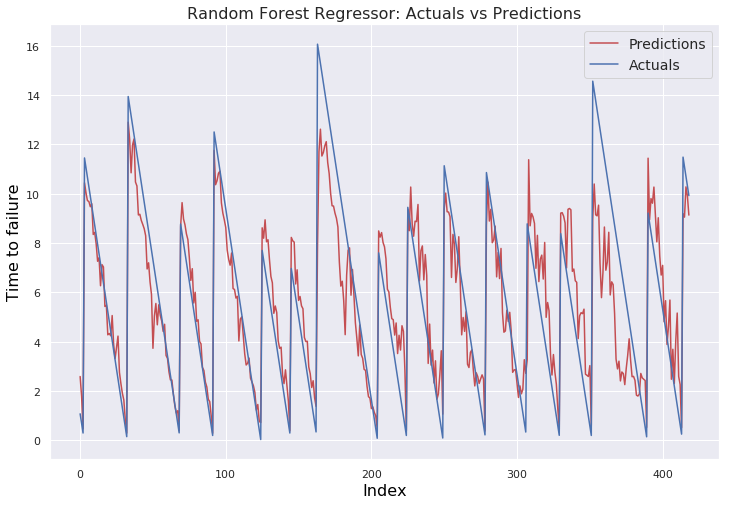
\includegraphics[width=.9\linewidth]{results1}
	\caption{Results achieved with Random Forest Regressor are 1.65 MAE and 0.63 $r^2$. We emphasize that there is no past or future information considered in calculating the predictions (red line). Each prediction uses only the acoustic signal information within one single time window.}
	\label{fig:results1}
\end{figure}


\begin{figure}
	\centering
	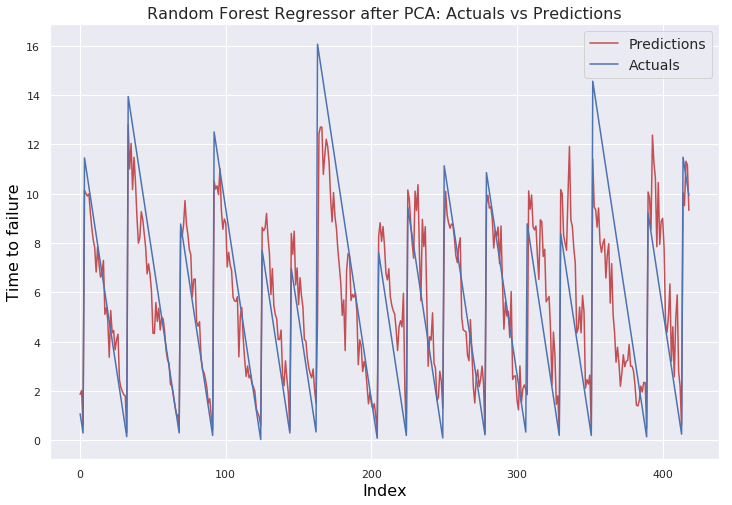
\includegraphics[width=.9\linewidth]{results1PCA}
	\caption{Random Forest Regressor after PCA MAE score is 1.78 and $r^2$ is 0.57.}
	\label{fig:results1PCA}
\end{figure}


\begin{figure}[H]
	\centering
	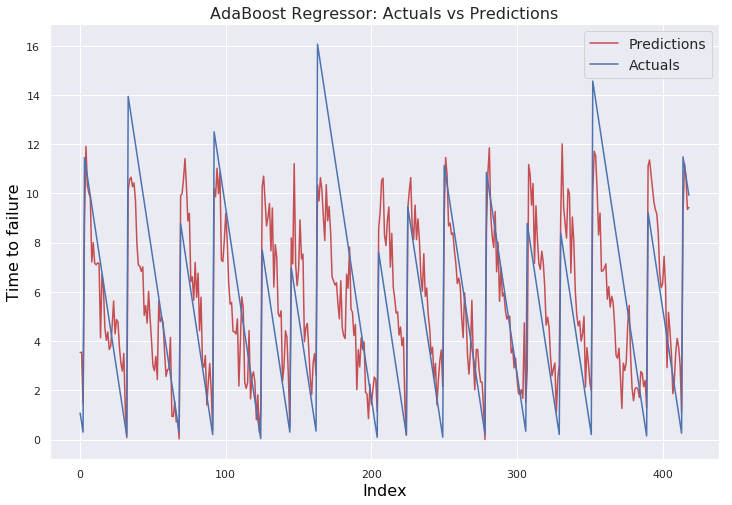
\includegraphics[width=.9\linewidth]{results2}
	\caption{Ada Boost Regressor MAE is 1.68 seconds and $r^2$ score is 0.62.}
	\label{fig:results2}
\end{figure}

\begin{figure}[H]
	\centering
	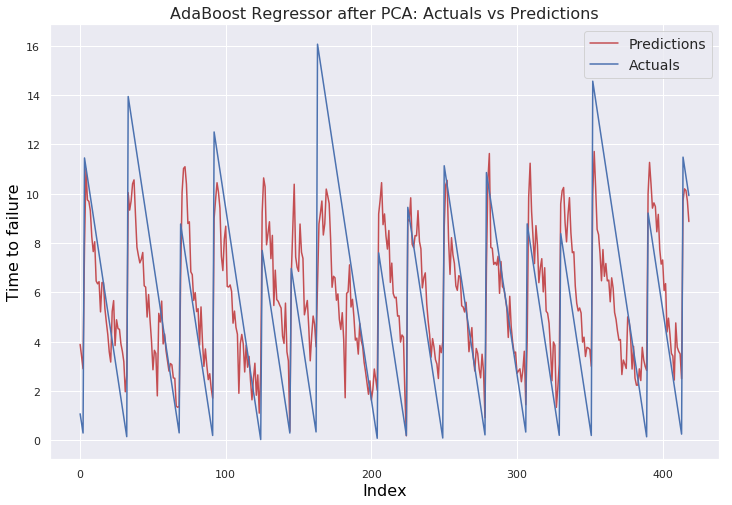
\includegraphics[width=.9\linewidth]{results2PCA}
	\caption{Ada Boost Regressor after PCA MAE score is 1.72 and $r^2$ is 0.63.}
	\label{fig:results2PCA}
\end{figure}


\clearpage
\newpage
\section{Analysis}
The most accurate results with coefficient of determination 0.63 and mean absolute error 1.65 seconds were achieved using the Random Forest algorithm. The most important features are shown on Figure 13. The top 4 are 90\% and 95\% quartile rolling standard deviations, standard deviation of rolling absolute mean and average rolling standard deviation.
The values of all 4 features grows as failure approaches. The highest picks we have just when failure appears.
%$SD = \sqrt{\frac{1}{N-1} \sum_{i=1}^N (x_i - \overline{x})^2}$
\begin{figure}[H]
	\centering
%	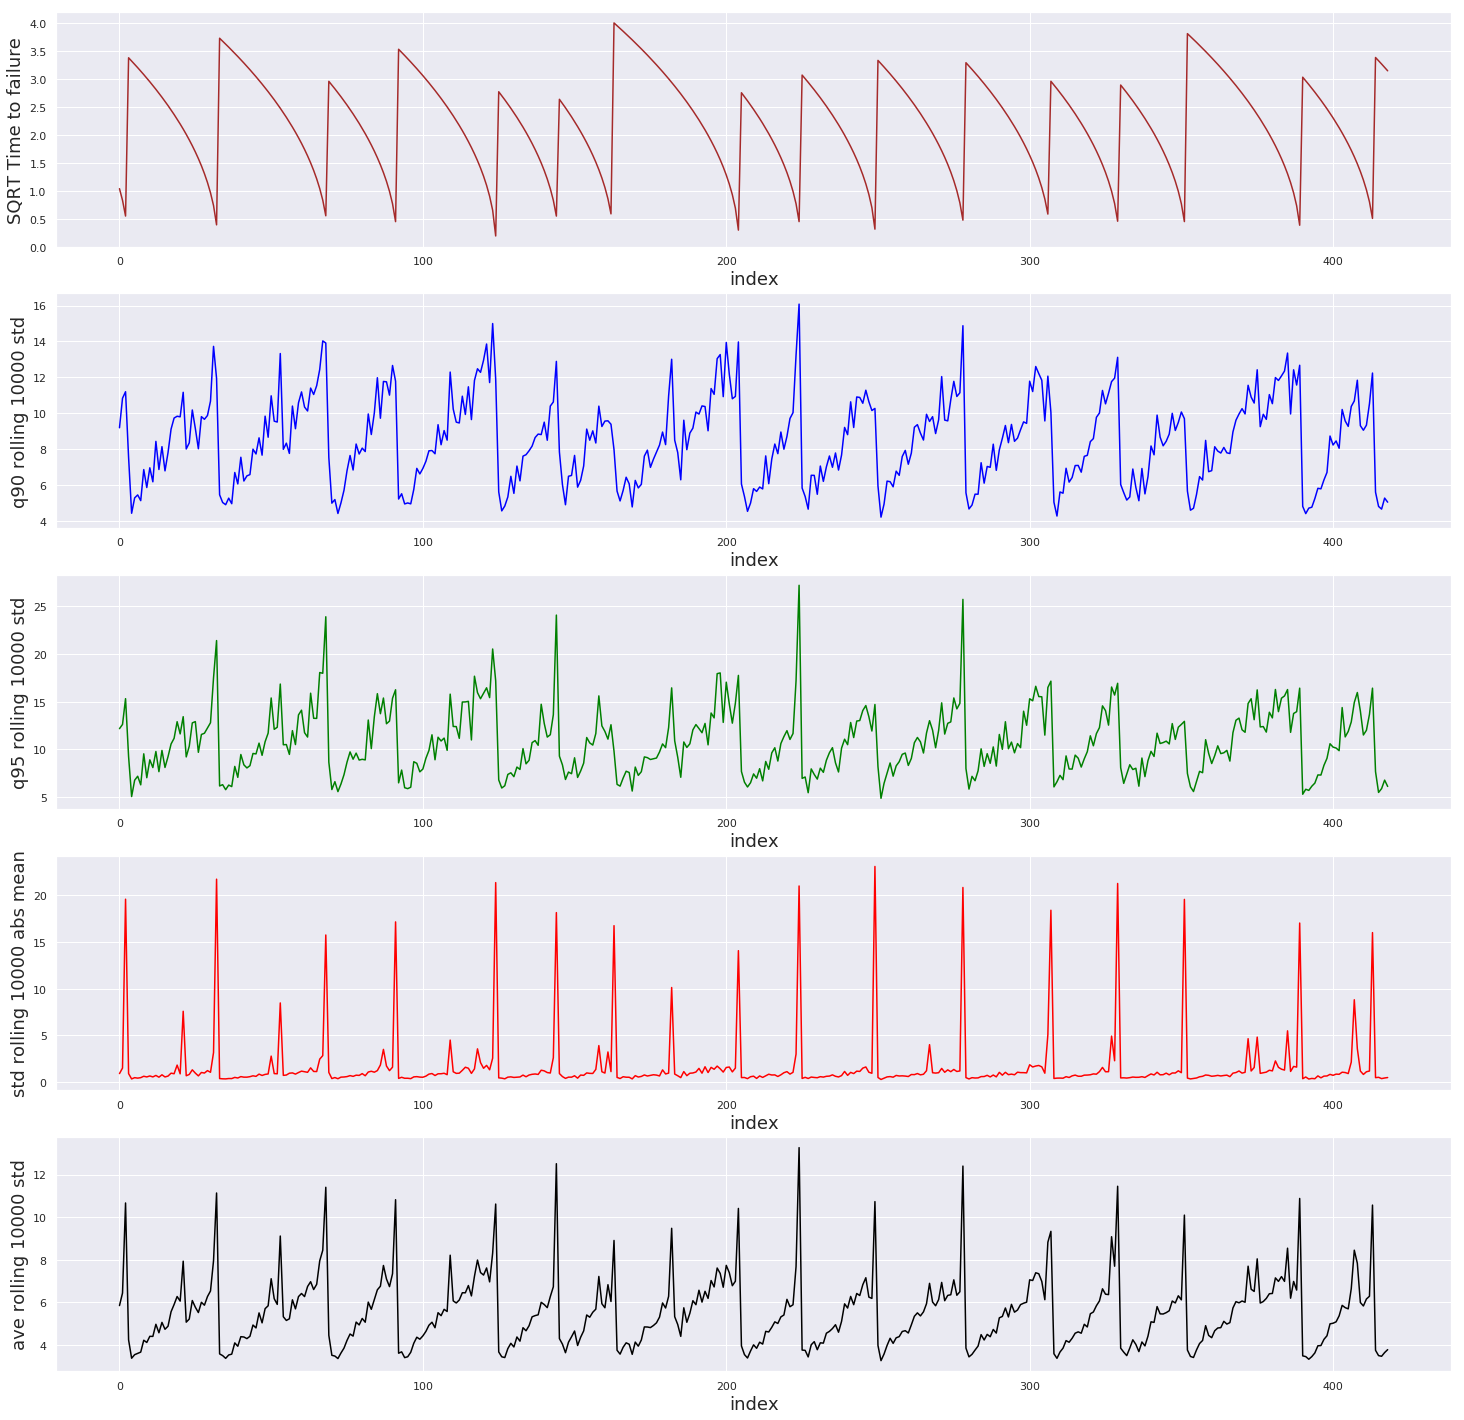
\includegraphics[width=14cm,height=14cm,keepaspectratio]{analysis}
	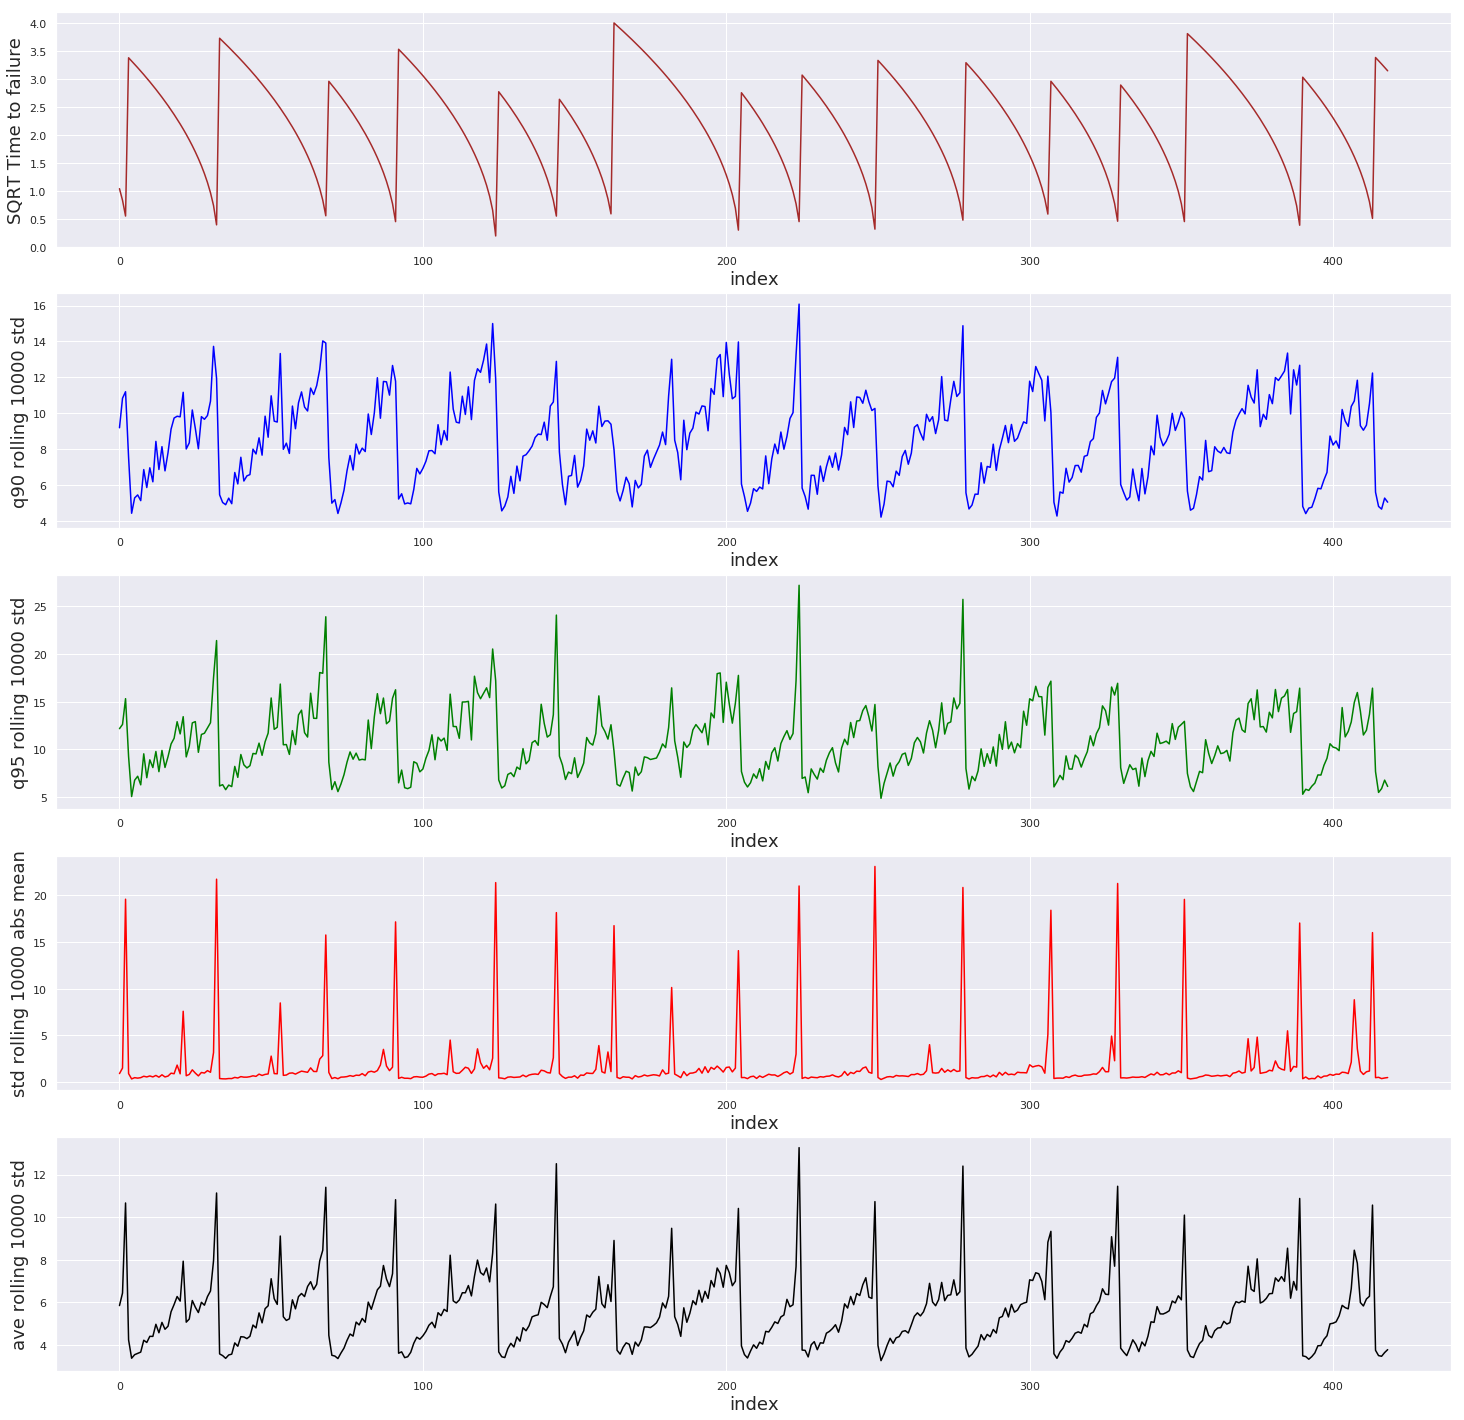
\includegraphics[width=1\linewidth]{analysis}
	\caption{The top 4 features in predicting time to failure}
	\label{fig:analysis}
\end{figure}

\clearpage
\newpage

\section{Ethics}

Our responsibility to report our results has to be weighed with our responsibility not to cause social disturbance. If the method demonstrated in this paper is scaled and applied to predict natural earthquakes this balance must be considered. Unwarranted predictions could have affects on personal property value while failure to report warranted predictions could result in loss of life or avoidable property damage. \par

Clarence R. Allen, the chairman of the National Earthquake Prediction Evaluation Council claimed that keeping information, from the public and discussing hypotheses on earthquake prediction “behind closed doors” would cause more harm than good, for free speech is the only means to promote research and to increase public responsibility of scientists \cite{Ayhan}. The public’s demand for accurate information would encourage scientists to further their research and hinder them from making unwarranted statements that may cause disturbance in society \cite{Ayhan}. Allen seems to suggest that free scientific communication in its due course would bring order to the scientific environment by eliminating unwarranted scientific hypotheses and predictions, together with the guesses of amateurs and cranks \cite{Ayhan}. \par
While the methods presented in this paper can eventually be scaled to real world earthquakes, it is unlikely that our findings will cause public disturbance as they apply only to \emph{laboratory} earthquakes. \par
In this study we follow the principles of the Association for Computing Machinery (ACM) Code of Ethics and Professional Conduct \cite{ACM} to ensure both privacy and security of individuals, and other codes of conduct related to good ethical practices. Ethical principles to make no harm, be honest and trustworthy, respect the work required to produce new ideas were used in our work. We also took professional responsibilities to achieve high quality in both the processes and professional work, maintain high standards of professional competence, accept and provide appropriate professional review, know and respect existing rules pertaining to professional work. \par

\section{Conclusions}

Given aperiodic earthquake failures data set with more akin to the observed behavior of natural earthquakes Random Forest Machine Learning technique can provide failure forecasts based on small windows of time. The acoustic signal measurement is an indicator of imminent failure. The prior recurrence interval is not needed to make a prediction. Predictions were made for time remaining before failure at any moment in the slip cycle.  The Random Forest machine learning technique provides the most accurate results. Predictions are based solely on acoustical signal's statistical features derived from the local, moving small time windows.\par
Feature engineering, size of the time window used in the model creation are essential to reduce mean absolute error. \par
%The results are another step toward learning the siesmic signals encouraging Machine Learning analysis of seismic signals in Earth.
%The results show that laboratory earthquakes can be predicted up to 16 seconds in advance.  \par
%
In this study we use only 157 seconds of the data that present 16 failures. Future work should introduce higher volumes of data to determine if accuracy can be improved. Also the combination of the acoustic signal and the recurrence interval should be tested to determine it's affect on accuracy.
\par
The results of our work are potentially applicable to the field of real world earthquakes \cite{Bertrand}. Essential improvements in providing new understanding of fault physics may be brought by applying this technique to acoustic seismic data. Other potential applications include avalanche prediction, landslides and failure of machine parts \cite{Bertrand}. \par

\section{Acknowledgment}
The authors thank Dr. Michael L. Blanpied, U.S. Geological Survey, for advice and reviews that greatly improved our work.

%References
\bibliographystyle{splncs}
\bibliography{myBibliography}

\end{document}
